\documentclass[aspectratio=169,11pt]{beamer}

\usepackage[utf8]{inputenc}
\usepackage[T1]{fontenc}
\usepackage{lmodern}
\usepackage{amsmath,amssymb,amsfonts}
\usepackage{mathtools}
\usepackage{booktabs}
\usepackage{graphicx}
\usepackage{tikz}
\usetikzlibrary{positioning,arrows.meta,calc}
\usepackage{ragged2e}
\usepackage{hyperref}
\usepackage{array}

\usetheme{default}
\useinnertheme{rectangles}

\definecolor{AcademicBlue}{RGB}{24,55,95}
\definecolor{SoftBlue}{RGB}{232,239,247}
\definecolor{DarkGray}{RGB}{55,55,55}
\definecolor{SolutionGreen}{RGB}{42,112,78}
\definecolor{SoftGreen}{RGB}{232,245,238}
\usetikzlibrary{arrows.meta,calc,angles,quotes}
\definecolor{VectorPurple}{RGB}{103,73,151}
\definecolor{DarkGray}{RGB}{55,55,55}
\definecolor{AxisGray}{RGB}{130,140,150}

\setbeamercolor{normal text}{fg=DarkGray,bg=white}
\setbeamercolor{structure}{fg=AcademicBlue}
\setbeamercolor{frametitle}{fg=AcademicBlue,bg=white}
\setbeamercolor{title}{fg=AcademicBlue}
\setbeamercolor{subtitle}{fg=DarkGray}
\setbeamercolor{block title}{fg=white,bg=AcademicBlue}
\setbeamercolor{block body}{fg=DarkGray,bg=SoftBlue}
\setbeamercolor{alerted text}{fg=AcademicBlue}
\setbeamercolor{example text}{fg=SolutionGreen}
\setbeamercolor{block title example}{fg=white,bg=SolutionGreen}
\setbeamercolor{block body example}{fg=DarkGray,bg=SoftGreen}

\setbeamerfont{title}{size=\LARGE,series=\bfseries}
\setbeamerfont{subtitle}{size=\normalsize}
\setbeamerfont{author}{size=\normalsize}
\setbeamerfont{institute}{size=\small}
\setbeamerfont{frametitle}{size=\large,series=\bfseries}
\setbeamerfont{block title}{series=\bfseries}
\setbeamersize{text margin left=0.55cm,text margin right=0.55cm}
\setbeamertemplate{navigation symbols}{}

\newcommand{\frontlogos}{%
    
\includegraphics[height=1.05cm]{logo-its.png}\hspace{0.22cm}%
    
\includegraphics[height=0.82cm]{logo-advancing-humanity.png}\hspace{0.22cm}%
    
\includegraphics[height=0.95cm]{logo-m.png}%
}

\newcommand{\slideMlogo}{%
    
\includegraphics[height=0.72cm]{logo-m.png}%
}

\newcommand{\source}[1]{%
    \vfill
    \hfill{\tiny\color{gray}Sumber: #1}
}

\newcommand{\axisgrid}[4]{%
    \draw[step=1cm,gray!20,very thin] (#1,#3) grid (#2,#4);
    \draw[-{Latex[length=2mm]},AcademicBlue,thick] (#1,0)--({#2+0.25},0) node[right] {$x$};
    \draw[-{Latex[length=2mm]},AcademicBlue,thick] (0,#3)--(0,{#4+0.25}) node[above] {$y$};
}

\setbeamertemplate{headline}{}

\setbeamertemplate{frametitle}{
    \vspace{0.15cm}
    \noindent\hbox to \textwidth{%
        \begin{minipage}[c]{0.86\textwidth}
            \raggedright
            \usebeamerfont{frametitle}
            \usebeamercolor[fg]{frametitle}
            \insertframetitle
        \end{minipage}%
        \hfill
        \begin{minipage}[c]{0.08\textwidth}
            \raggedleft
            \slideMlogo
        \end{minipage}%
    }
    \vspace{-0.05cm}
    {\color{AcademicBlue}\rule{\textwidth}{0.6pt}}
    \vspace{0.15cm}
}

\setbeamertemplate{footline}{
    \leavevmode
    \hbox{
        \begin{beamercolorbox}[
            wd=.75\paperwidth,
            ht=2.8ex,
            dp=1.2ex,
            leftskip=0.5cm
        ]{normal text}
        \scriptsize \insertshorttitle
        \end{beamercolorbox}
        \begin{beamercolorbox}[
            wd=.25\paperwidth,
            ht=2.8ex,
            dp=1.2ex,
            rightskip=0.5cm plus1fil
        ]{normal text}
        \hfill\scriptsize \insertframenumber/\inserttotalframenumber
        \end{beamercolorbox}
    }
}

\setbeamertemplate{itemize item}{\color{AcademicBlue}\small$\blacksquare$}
\setbeamertemplate{itemize subitem}{\color{AcademicBlue}\scriptsize$\blacktriangleright$}

\AtBeginSection[]{
    \begin{frame}
        \vfill
        \begin{center}
            {\color{AcademicBlue}\Large\bfseries \insertsection}
            \vspace{0.3cm}

            {\color{AcademicBlue}\rule{0.35\textwidth}{0.8pt}}
        \end{center}
        \vfill
    \end{frame}
}

\title[Topik Aljabar Terapan -- Pertemuan 1]{Topik Aljabar Terapan (SM255213)}
\subtitle{\Large Introduction}
\author{}
\institute{
    Departemen Matematika\\
    Institut Teknologi Sepuluh Nopember
}
\date{Pertemuan 1}

\begin{document}

% 1
\begin{frame}[plain]
    \vspace{0.15cm}
    \begin{flushleft}
        \frontlogos
    \end{flushleft}
    \vspace{0.50cm}
    {\color{AcademicBlue}\rule{\textwidth}{1.2pt}}
    \vspace{0.50cm}

    {\usebeamerfont{title}\color{AcademicBlue}\inserttitle\par}
    \vspace{0.25cm}
    {\usebeamerfont{subtitle}\insertsubtitle\par}
    \vspace{0.50cm}

    {\usebeamerfont{author}\textbf{\insertauthor}\par}
    \vspace{0.15cm}
    {\usebeamerfont{institute}\insertinstitute\par}
    \vspace{0.35cm}
    {\small\insertdate}
    \vfill
\end{frame}

% 2
\begin{frame}{Are quantum computers possible?}
    \begin{itemize}
		\item Classical computation operates on \textit{bits}, but quantum computation operates on \textit{qubits}
		\item Such question is yet to be resolved
		\item Fortunately, the question does not pose a barrier to us: we plan to study \textbf{quantum algorithms}
		\item The mathematics required to understand them is linear algebra: vectors, matrices, and their basic properties
	\end{itemize}
    
\end{frame}

% 3
\begin{frame}{The model: the space and the states}
    \begin{itemize}
		\item The state is described by a single unit vector $\mathbf{a} = \begin{bmatrix} a_0 & \dots & a_{N-1}\end{bmatrix}^T$ that lies in some fixed vector space of dimension $N = 2^n$, for some $n$, where each entry $a_k$ is a real or complex number
		\item Each entry is called an \textbfamplitude}
		\item In the \textbf{standard basis}, the basis states are denoted by the vectors $\mathbf{e}_k$
		\item We further identify $k$ with the $k$-th string $x$ in a fixed total ordering of $\{0,1\}^n$
		\item Since basis states correspond to all the length-$n$ binary strings, we have $N = 2^n$
	\end{itemize}
\end{frame}

% 4
%\begin{frame}{Capaian pembelajaran pertemuan}
%    Setelah mengikuti pertemuan ini, mahasiswa mampu:
%    \begin{enumerate}
%        \item mendefinisikan sistem koordinat rectangular dan oblique;
%        \item menentukan koordinat dan kedudukan titik pada bidang;
%        \item membuktikan rumus jarak, titik tengah, dan titik pembagi ruas;
%        \item membentuk persamaan grafik dan tempat kedudukan sederhana.
%    \end{enumerate}
%    \source{RPS Geometri Analitik SM234102}
%\end{frame}

\section{Sistem Koordinat dan Kedudukan Titik}

% 6
\begin{frame}{Koordinat adalah representasi tunggal suatu titik}
    \begin{columns}[c]
        \column{0.53\textwidth}
        \centering
        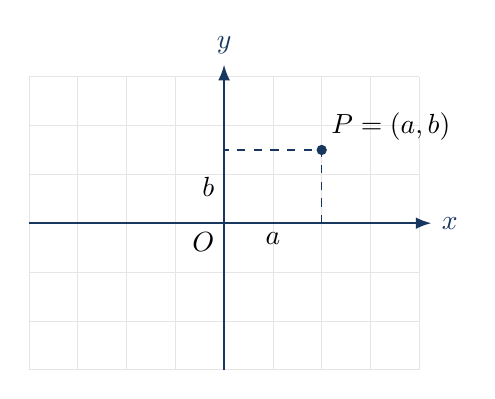
\begin{tikzpicture}[scale=0.62]
            \axisgrid{-4}{4}{-3}{3}
            \fill[AcademicBlue] (2,1.5) circle (3pt);
            \draw[dashed,AcademicBlue] (2,0)--(2,1.5)--(0,1.5);
            \node[above right] at (2,1.5) {$P=(a,b)$};
            \node[below left] at (0,0) {$O$};
            \node[below] at (1,0) {$a$};
            \node[left] at (0,0.75) {$b$};
        \end{tikzpicture}

        \column{0.43\textwidth}
        \begin{block}{Definisi}
            \begin{itemize}
                \item $a$ disebut \textbf{absis};
                \item $b$ disebut \textbf{ordinat};
                \item $(a,b)$ disebut koordinat $P$;
                \item $O=(0,0)$ disebut titik asal.
            \end{itemize}
        \end{block}
    \end{columns}

    Secara matematis, setiap $P$ pada bidang berkorespondensi tepat dengan satu
    pasangan $(a,b)\in\mathbb{R}^2$.
    
\end{frame}

% 7
\begin{frame}{Tanda koordinat menentukan kedudukan titik}
    \begin{columns}[c]
        \column{0.49\textwidth}
        \centering
        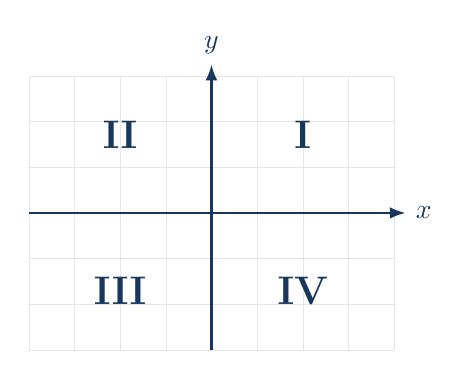
\begin{tikzpicture}[scale=0.58]
            \axisgrid{-4}{4}{-3}{3}
            \node[font=\Large\bfseries,text=AcademicBlue] at (2,1.7) {I};
            \node[font=\Large\bfseries,text=AcademicBlue] at (-2,1.7) {II};
            \node[font=\Large\bfseries,text=AcademicBlue] at (-2,-1.7) {III};
            \node[font=\Large\bfseries,text=AcademicBlue] at (2,-1.7) {IV};
        \end{tikzpicture}

        \column{0.47\textwidth}
        \renewcommand{\arraystretch}{1.20}
        \begin{tabular}{c@{\qquad}c}
            \toprule
            Kedudukan & Syarat tanda\\
            \midrule
            Kuadran I   & $x>0,\ y>0$\\
            Kuadran II  & $x<0,\ y>0$\\
            Kuadran III & $x<0,\ y<0$\\
            Kuadran IV  & $x>0,\ y<0$\\
            Sumbu $x$   & $y=0$\\
            Sumbu $y$   & $x=0$\\
            \bottomrule
        \end{tabular}
    \end{columns}
    
\end{frame}


% 9
\begin{frame}{Latihan 1 -- Kedudukan titik}
    \begin{block}{Soal}
        Tentukan kedudukan setiap titik berikut: kuadran I, II, III, IV,
        sumbu $x$, sumbu $y$, atau titik asal.
        \[
            A=(3,2),\quad B=(-2,4),\quad C=(-3,-1),
        \]
        \[
            D=(2,-3),\quad E=(0,5),\quad F=(-4,0),\quad G=(0,0).
        \]
    \end{block}
    \vspace{0.35cm}
    \centering
%    \color{AcademicBlue}\bfseries Gunakan definisi tanda koordinat, bukan hanya gambar.
\end{frame}

% 10
\begin{frame}{Latihan 1 -- Soal dan pembahasan}
    \begin{exampleblock}{Soal}
        Tentukan kedudukan $A,B,C,D,E,F$, dan $G$ berdasarkan tanda koordinatnya.
    \end{exampleblock}

    \renewcommand{\arraystretch}{1.15}
    \centering
    \begin{tabular}{c@{\quad}c@{\quad}l}
        \toprule
        Titik & Tanda & Kedudukan\\
        \midrule
        $A=(3,2)$ & $(+,+)$ & kuadran I\\
        $B=(-2,4)$ & $(-,+)$ & kuadran II\\
        $C=(-3,-1)$ & $(-,-)$ & kuadran III\\
        $D=(2,-3)$ & $(+,-)$ & kuadran IV\\
        $E=(0,5)$ & $(0,+)$ & sumbu $y$\\
        $F=(-4,0)$ & $(-,0)$ & sumbu $x$\\
        $G=(0,0)$ & $(0,0)$ & titik asal\\
        \bottomrule
    \end{tabular}
\end{frame}
% 8
\begin{frame}{Sudut antarsumbu membedakan dua sistem koordinat}
	\vspace{-1cm}
	Misalkan $\mathbf e_1$ dan $\mathbf e_2$ adalah vektor satuan sepanjang dua
	sumbu dan $\omega$ adalah sudut di antara keduanya. Posisi titik dinyatakan oleh
	\[
	\overrightarrow{OP}=x\mathbf e_1+y\mathbf e_2.
	\]
	
	\begin{columns}[T]
		\column{0.46\textwidth}
		\begin{block}{Sistem Oblique}
			$\omega$ tidak harus $90^\circ$. Akibatnya,
			$\mathbf e_1\cdot\mathbf e_2=\cos\omega$ mungkin tidak nol.
		\end{block}
		
		\column{0.46\textwidth}
		\begin{block}{Sistem Rectangular}
			$\omega=90^\circ$, sehingga
			$\mathbf e_1\cdot\mathbf e_2=0$. Kedua sumbu saling ortogonal.
		\end{block}
	\end{columns}
	
\end{frame}
\begin{frame}
	\resizebox{0.95\textwidth}{!}{%
	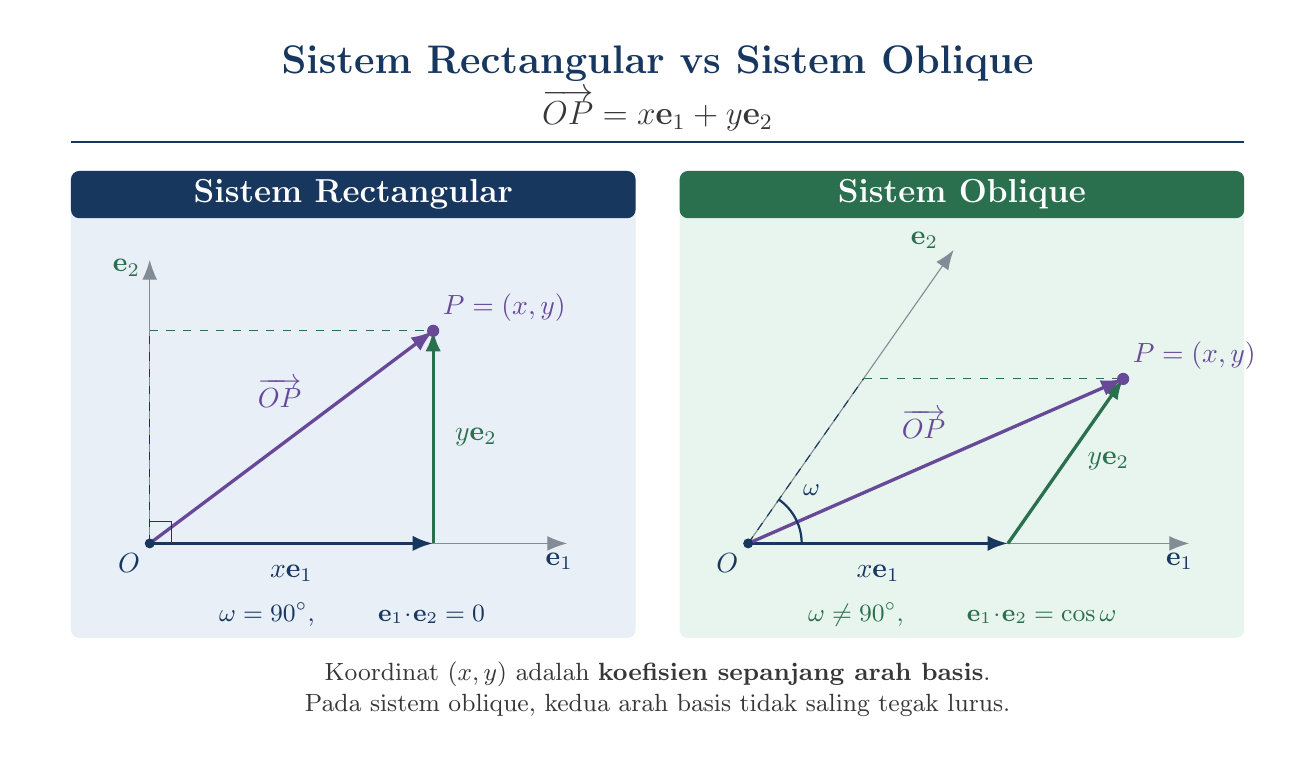
\begin{tikzpicture}[x=1cm,y=1cm,>=Latex,font=\sffamily,text=DarkGray]
		\useasboundingbox (0,0) rectangle (16,9);
		\fill[white] (0,0) rectangle (16,9);
		
		% Judul dan persamaan utama
		\node[font=\bfseries\Large,text=AcademicBlue] at (8,8.55)
		{Sistem Rectangular vs Sistem Oblique};
		\node[font=\large] at (8,7.95)
		{$\overrightarrow{OP}=x\mathbf e_1+y\mathbf e_2$};
		\draw[AcademicBlue,line width=0.6pt] (0.55,7.55)--(15.45,7.55);
		
		% Panel rectangular
		\fill[SoftBlue,rounded corners=3pt] (0.55,1.25) rectangle (7.72,7.18);
		\fill[AcademicBlue,rounded corners=3pt] (0.55,6.58) rectangle (7.72,7.18);
		\node[font=\bfseries\large,text=white] at (4.135,6.88)
		{Sistem Rectangular};
		
		\coordinate (OR) at (1.55,2.45);
		\coordinate (AR) at (5.15,2.45);
		\coordinate (BR) at (1.55,5.15);
		\coordinate (PR) at (5.15,5.15);
		
		% sumbu/basis rectangular
		\draw[AxisGray,thin,-{Latex[length=2.5mm]}] (OR)--(6.85,2.45);
		\draw[AxisGray,thin,-{Latex[length=2.5mm]}] (OR)--(1.55,6.05);
		\draw[AcademicBlue,very thick,-{Latex[length=2.6mm]}] (OR)--(AR)
		node[midway,below=4pt] {$x\mathbf e_1$};
		\draw[SolutionGreen,very thick,-{Latex[length=2.6mm]}] (AR)--(PR)
		node[midway,right=4pt] {$y\mathbf e_2$};
		\draw[AcademicBlue,dashed] (OR)--(BR);
		\draw[SolutionGreen,dashed] (BR)--(PR);
		\draw[VectorPurple,line width=1.2pt,-{Latex[length=2.8mm]}] (OR)--(PR)
		node[pos=0.58,above left=1pt] {$\overrightarrow{OP}$};
		
		\fill[AcademicBlue] (OR) circle (1.8pt) node[below left] {$O$};
		\fill[VectorPurple] (PR) circle (2.2pt) node[above right] {$P=(x,y)$};
		\node[below,text=AcademicBlue] at (6.75,2.45) {$\mathbf e_1$};
		\node[left,text=SolutionGreen] at (1.55,5.95) {$\mathbf e_2$};
		\draw[AcademicBlue] ($(OR)+(0.28,0)$)--($(OR)+(0.28,0.28)$)--($(OR)+(0,0.28)$);
		\node[font=\small\bfseries,text=AcademicBlue] at (4.12,1.55)
		{$\omega=90^\circ,\qquad \mathbf e_1\!\cdot\!\mathbf e_2=0$};
		
		% Panel oblique
		\fill[SoftGreen,rounded corners=3pt] (8.28,1.25) rectangle (15.45,7.18);
		\fill[SolutionGreen,rounded corners=3pt] (8.28,6.58) rectangle (15.45,7.18);
		\node[font=\bfseries\large,text=white] at (11.865,6.88)
		{Sistem Oblique};
		
		\coordinate (OO) at (9.15,2.45);
		\coordinate (AO) at (12.45,2.45);
		\coordinate (BO) at ($(OO)+(55:2.55)$);
		\coordinate (PO) at ($(AO)+(55:2.55)$);
		
		% sumbu/basis oblique
		\draw[AxisGray,thin,-{Latex[length=2.5mm]}] (OO)--(14.75,2.45);
		\draw[AxisGray,thin,-{Latex[length=2.5mm]}] (OO)--($(OO)+(55:4.55)$);
		\draw[AcademicBlue,very thick,-{Latex[length=2.6mm]}] (OO)--(AO)
		node[midway,below=4pt] {$x\mathbf e_1$};
		\draw[SolutionGreen,very thick,-{Latex[length=2.6mm]}] (AO)--(PO)
		node[midway,right=4pt] {$y\mathbf e_2$};
		\draw[AcademicBlue,dashed] (OO)--(BO);
		\draw[SolutionGreen,dashed] (BO)--(PO);
		\draw[VectorPurple,line width=1.2pt,-{Latex[length=2.8mm]}] (OO)--(PO)
		node[pos=0.56,above left=1pt] {$\overrightarrow{OP}$};
		
		\fill[AcademicBlue] (OO) circle (1.8pt) node[below left] {$O$};
		\fill[VectorPurple] (PO) circle (2.2pt) node[above right] {$P=(x,y)$};
		\node[below,text=AcademicBlue] at (14.63,2.45) {$\mathbf e_1$};
		\node[above left,text=SolutionGreen] at ($(OO)+(55:4.42)$) {$\mathbf e_2$};
		
		\draw[AcademicBlue,thick] ($(OO)+(0.68,0)$) arc[start angle=0,end angle=55,radius=0.68];
		\node[font=\small,text=AcademicBlue] at ($(OO)+(40:1.05)$) {$\omega$};
		\node[font=\small\bfseries,text=SolutionGreen] at (11.87,1.55)
		{$\omega\neq90^\circ,\qquad \mathbf e_1\!\cdot\!\mathbf e_2=\cos\omega$};
		
		% Catatan konseptual
		\fill[white,rounded corners=2pt] (2.15,0.25) rectangle (13.85,0.95);
		\node[align=center,font=\small] at (8,0.60) {Koordinat $(x,y)$ adalah \textbf{koefisien sepanjang arah basis}.\\
			Pada sistem oblique, kedua arah basis tidak saling tegak lurus.};
	\end{tikzpicture}}
\end{frame}

\section{Relasi Analitik Antar Titik}

% 12
\begin{frame}{Selisih koordinat menyatakan perpindahan}
    Untuk $P_1=(x_1,y_1)$ dan $P_2=(x_2,y_2)$, definisikan
    \[
        \Delta x=x_2-x_1,
        \qquad
        \Delta y=y_2-y_1.
    \]
    Pada sistem rectangular,
    \[
        \overrightarrow{P_1P_2}=(\Delta x,\Delta y).
    \]

    \begin{alertblock}{Interpretasi}
        Nilai $\Delta x$ dan $\Delta y$ adalah besaran bertanda. Tandanya
        menyatakan arah, sedangkan nilai mutlaknya menyatakan panjang proyeksi.
    \end{alertblock}
    
\end{frame}

% 13
\begin{frame}{Teorema 1 -- Rumus jarak pada bidang rectangular}
    \begin{block}{Teorema}
        Jika $P_1=(x_1,y_1)$ dan $P_2=(x_2,y_2)$ berada pada bidang rectangular,
        maka
        \[
            \boxed{d(P_1,P_2)=
            \sqrt{(x_2-x_1)^2+(y_2-y_1)^2}}.
        \]
    \end{block}

    \begin{alertblock}{Sifat}
        $d(P_1,P_2)\ge 0$, simetris, dan $d(P_1,P_2)=0$ jika dan hanya jika
        $P_1=P_2$.
    \end{alertblock}
    
\end{frame}

% 14
\begin{frame}{Bukti :}
    \begin{columns}[c]
        \column{0.49\textwidth}
        \centering
        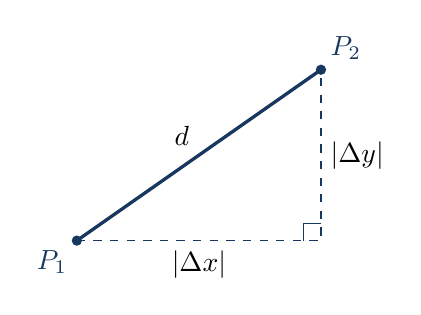
\begin{tikzpicture}[scale=0.62]
            \coordinate (Pone) at (-2,-1);
            \coordinate (Ptwo) at (3,2.5);
            \coordinate (Q) at (3,-1);
            \draw[AcademicBlue,very thick] (Pone)--(Ptwo);
            \draw[dashed,AcademicBlue] (Pone)--(Q)--(Ptwo);
            \draw[AcademicBlue] ($(Q)+(-0.35,0)$)--($(Q)+(-0.35,0.35)$)--($(Q)+(0,0.35)$);
            \fill[AcademicBlue] (Pone) circle (3pt) node[below left] {$P_1$};
            \fill[AcademicBlue] (Ptwo) circle (3pt) node[above right] {$P_2$};
            \node[below] at (0.5,-1) {$|\Delta x|$};
            \node[right] at (3,0.75) {$|\Delta y|$};
            \node[above left] at (0.5,0.75) {$d$};
        \end{tikzpicture}

        \column{0.47\textwidth}
        Segitiga $P_1QP_2$ siku-siku di $Q$, sehingga
        \[
            d^2=|\Delta x|^2+|\Delta y|^2.
        \]
        Karena $|a|^2=a^2$,
        \[
            d^2=(x_2-x_1)^2+(y_2-y_1)^2.
        \]
        Ambil akar tak negatif pada kedua ruas untuk memperoleh rumus teorema.
        \hfill$\square$
    \end{columns}
\end{frame}

% 15
\begin{frame}{Teorema 2 -- Rumus jarak pada bidang oblique}
    \begin{block}{Teorema}
        Jika sudut antarsumbu adalah $\omega$, maka
        \[
            \boxed{d^2=(\Delta x)^2+(\Delta y)^2
            +2(\Delta x)(\Delta y)\cos\omega}.
        \]
    \end{block}

    Rumus ini memuat suku silang karena kedua arah sumbu tidak selalu ortogonal.
    \begin{alertblock}{Kasus khusus}
        Untuk $\omega=90^\circ$, $\cos\omega=0$ dan Teorema 2 mereduksi menjadi
        Teorema 1.
    \end{alertblock}
    
\end{frame}

% 16
\begin{frame}{Bukti : menggunakan hasil kali dalam}
    Tuliskan vektor perpindahan sebagai
    \[
        \mathbf v=\Delta x\,\mathbf e_1+\Delta y\,\mathbf e_2,
    \]
    dengan $\|\mathbf e_1\|=\|\mathbf e_2\|=1$ dan
    $\mathbf e_1\cdot\mathbf e_2=\cos\omega$. Maka
    \[
    \begin{aligned}
        d^2=\|\mathbf v\|^2
        &=\mathbf v\cdot\mathbf v\\
        &=(\Delta x)^2\|\mathbf e_1\|^2
          +(\Delta y)^2\|\mathbf e_2\|^2
          +2(\Delta x)(\Delta y)(\mathbf e_1\cdot\mathbf e_2)\\
        &=(\Delta x)^2+(\Delta y)^2
          +2(\Delta x)(\Delta y)\cos\omega.
    \end{aligned}
    \]
    Dengan demikian rumus pada Teorema 2 terbukti. \hfill$\square$
\end{frame}

% 17
\begin{frame}{Latihan 2 -- Jarak pada dua sistem koordinat}
    \begin{block}{Soal}
        Diberikan $A=(-2,1)$ dan $B=(4,-7)$.
        \begin{enumerate}
            \item Hitung $AB$ jika sumbu koordinat saling tegak lurus.
            \item Hitung $AB$ jika sudut antarsumbu adalah $60^\circ$.
        \end{enumerate}
    \end{block}

    \vspace{0.35cm}
    \centering
    \color{AcademicBlue}\bfseries Gunakan $\Delta x=6$, $\Delta y=-8$, dan perhatikan tanda suku silang.
\end{frame}

% 18
\begin{frame}{Latihan 2 -- Soal dan pembahasan}
    \begin{exampleblock}{Soal}
        Hitung jarak $A=(-2,1)$ dan $B=(4,-7)$ pada sistem rectangular dan
        sistem oblique dengan $\omega=60^\circ$.
    \end{exampleblock}

    \begin{enumerate}
        \item Sistem rectangular:
        \[
            AB=\sqrt{6^2+(-8)^2}=\sqrt{100}=\boxed{10}.
        \]
        \item Sistem oblique:
        \[
        \begin{aligned}
            AB^2&=6^2+(-8)^2+2(6)(-8)\cos60^\circ\\
                &=36+64-48=52,
        \end{aligned}
        \]
        sehingga $AB=\boxed{2\sqrt{13}}$.
    \end{enumerate}
\end{frame}

% 19
\begin{frame}{Teorema 3 -- Koordinat titik tengah}
    \begin{block}{Teorema}
        Jika $M$ adalah titik tengah ruas $P_1P_2$, dengan
        $P_1=(x_1,y_1)$ dan $P_2=(x_2,y_2)$, maka
        \[
            \boxed{M=\left(\frac{x_1+x_2}{2},
            \frac{y_1+y_2}{2}\right)}.
        \]
    \end{block}

    Secara vektorial,
    \[
        \overrightarrow{OM}=\frac12\left(
        \overrightarrow{OP_1}+\overrightarrow{OP_2}\right).
    \]
    
\end{frame}

% 20
\begin{frame}{Bukti :}
    Misalkan $M=(x_M,y_M)$. Karena $M$ adalah titik tengah, perpindahan
    dari $P_1$ ke $M$ sama dengan perpindahan dari $M$ ke $P_2$:
    \[
        \overrightarrow{P_1M}=\overrightarrow{MP_2}.
    \]
    Maka
    \[
        (x_M-x_1,\ y_M-y_1)=(x_2-x_M,\ y_2-y_M).
    \]
    Kesamaan komponen memberikan
    \[
        2x_M=x_1+x_2,
        \qquad
        2y_M=y_1+y_2.
    \]
    Jadi
    \[
        M=\left(\frac{x_1+x_2}{2},\frac{y_1+y_2}{2}\right).
        \qquad\square
    \]
\end{frame}

% 21
\begin{frame}{Latihan 3 -- Titik tengah ruas garis}
    \begin{block}{Soal}
        Diberikan $A=(-5,4)$ dan $B=(3,-2)$.
        \begin{enumerate}
            \item Tentukan titik tengah $M$ dari ruas $AB$.
            \item Verifikasi bahwa $AM=MB$ menggunakan Teorema 1.
        \end{enumerate}
    \end{block}
    \vspace{0.35cm}
    \centering
    \color{AcademicBlue}\bfseries Pembuktian numerik harus konsisten dengan definisi titik tengah.
\end{frame}

% 22
\begin{frame}{Latihan 3 -- Soal dan pembahasan}
    \begin{exampleblock}{Soal}
        Tentukan titik tengah ruas $A=(-5,4)$ dan $B=(3,-2)$, lalu verifikasi panjangnya.
    \end{exampleblock}

    \[
        M=\left(\frac{-5+3}{2},\frac{4-2}{2}\right)=\boxed{(-1,1)}.
    \]
    Selanjutnya,
    \[
    \begin{aligned}
        AM&=\sqrt{(-1+5)^2+(1-4)^2}=\sqrt{4^2+(-3)^2}=5,\\
        MB&=\sqrt{(3+1)^2+(-2-1)^2}=\sqrt{4^2+(-3)^2}=5.
    \end{aligned}
    \]
    Dengan demikian $AM=MB$, sesuai definisi titik tengah.
\end{frame}

% 23
\begin{frame}{Teorema 4 -- Koordinat titik pembagi diantara dua titik}
    \begin{block}{Teorema}
        Jika $P$ membagi ruas $P_1P_2$ secara internal dengan
        \[
            P_1P:PP_2=m:n,
        \]
        maka
        \[
            \boxed{P=\left(\frac{nx_1+mx_2}{m+n},
            \frac{ny_1+my_2}{m+n}\right)}.
        \]
    \end{block}

    Koefisien setiap titik merupakan bobot dari bagian ruas yang berseberangan.
    
\end{frame}

% 24
\begin{frame}{Bukti Teorema 4 menggunakan kombinasi afin}
    Karena $P_1P:PP_2=m:n$, proporsi posisi $P$ dari $P_1$ menuju $P_2$ adalah
    \[
        t=\frac{P_1P}{P_1P+PP_2}=\frac{m}{m+n}.
    \]
    Oleh karena itu,
    \[
        \overrightarrow{OP}
        =(1-t)\overrightarrow{OP_1}+t\overrightarrow{OP_2}.
    \]
    Substitusi $t=m/(m+n)$ menghasilkan
    \[
    \begin{aligned}
        \overrightarrow{OP}
        &=\frac{n}{m+n}(x_1,y_1)+\frac{m}{m+n}(x_2,y_2)\\
        &=\left(\frac{nx_1+mx_2}{m+n},
        \frac{ny_1+my_2}{m+n}\right).
    \end{aligned}
    \]
    Jadi rumus titik pembagi internal terbukti. \hfill$\square$
\end{frame}

% 25
\begin{frame}{Latihan 4 -- Pembagian ruas dengan rasio}
    \begin{block}{Soal}
        Titik $P$ membagi ruas dari $P_1=(6,1)$ ke $P_2=(-2,9)$ secara internal
        dengan rasio
        \[
            P_1P:PP_2=3:5.
        \]
        Tentukan koordinat $P$ dan parameter afin $t$.
    \end{block}
    \vspace{0.35cm}
    \centering
    \color{AcademicBlue}\bfseries Tentukan dahulu $m$, $n$, dan $t=m/(m+n)$.
\end{frame}

% 26
\begin{frame}{Latihan 4 -- Soal dan pembahasan}
    \begin{exampleblock}{Soal}
        Tentukan titik pembagi $P_1=(6,1)$ dan $P_2=(-2,9)$ dengan rasio $3:5$.
    \end{exampleblock}

    Diperoleh $m=3$, $n=5$, dan $t=3/8$. Dengan Teorema 4,
    \[
    \begin{aligned}
        x_P&=\frac{5(6)+3(-2)}{8}=3,\\
        y_P&=\frac{5(1)+3(9)}{8}=4.
    \end{aligned}
    \]
    Jadi
    \[
        \boxed{P=(3,4)}.
    \]
    Pemeriksaan: $P=P_1+\frac38(P_2-P_1)=(6,1)+\frac38(-8,8)=(3,4)$.
\end{frame}

\section{Persamaan Grafik dan Tempat Kedudukan}

% 28
\begin{frame}{Grafik dan locus dinyatakan melalui ekuivalensi}
    \begin{block}{Dua definisi himpunan}
        Grafik persamaan $F(x,y)=0$ dan locus dengan sifat geometris
        $\mathcal S$ berturut-turut ialah
        \[
            G=\{(x,y)\in\mathbb R^2\mid F(x,y)=0\},\qquad
            L=\{P\in\mathbb R^2\mid P\text{ memenuhi }\mathcal S\}.
        \]
    \end{block}

    Persamaan $F(x,y)=0$ merepresentasikan locus secara tepat apabila
    \[
        P\text{ memenuhi }\mathcal S
        \quad\Longleftrightarrow\quad F(x,y)=0.
    \]
    
\end{frame}

% 29
\begin{frame}{Proposisi 1 -- Bisektor $y=x$}
    \begin{block}{Proposisi}
        Himpunan titik dengan absis dan ordinat sama ialah garis
        $\boxed{y=x}$, yaitu bisektor sudut sumbu koordinat pada kuadran I dan III.
    \end{block}

    \centering
    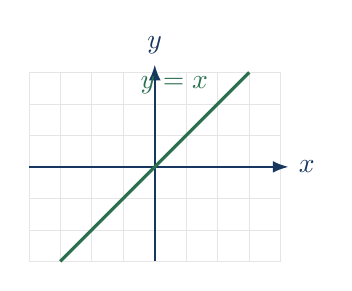
\begin{tikzpicture}[scale=0.40]
        \axisgrid{-4}{4}{-3}{3}
        \draw[SolutionGreen,very thick] (-3,-3)--(3,3);
        \node[above left,text=SolutionGreen] at (2,2) {$y=x$};
    \end{tikzpicture}
    \source{Fahim (2022); Riddle (1982)}
\end{frame}

% 30
\begin{frame}{Bukti Proposisi 1 menggunakan dua implikasi}
    Misalkan $P=(x,y)$.
    \begin{enumerate}
        \item Jika $P$ terletak pada bisektor kuadran I atau III, maka jarak
        bertanda $P$ terhadap kedua sumbu sama. Akibatnya $x=y$.
        \item Sebaliknya, jika $x=y$, maka
        \[
            P=(x,x)=x(1,1).
        \]
        Jadi $P$ terletak pada garis melalui $O$ dengan vektor arah $(1,1)$.
        Vektor ini membentuk sudut $45^\circ$ terhadap kedua sumbu.
    \end{enumerate}

    Dengan demikian,
    \[
        P\text{ berada pada bisektor}
        \quad\Longleftrightarrow\quad y=x.
        \qquad\square
    \]
\end{frame}

% 31
\begin{frame}{Teorema 5 -- Persamaan lingkaran dari definisi jarak}
    \begin{block}{Teorema}
        Locus titik $P=(x,y)$ yang berjarak tetap $r>0$ dari
        $C=(a,b)$ adalah lingkaran
        \[
            \boxed{(x-a)^2+(y-b)^2=r^2}.
        \]
    \end{block}

    Untuk $C=(0,0)$ dan $r=5$, diperoleh
    \[
        x^2+y^2=25.
    \]
    \begin{alertblock}{Makna}
        Titik $P$ boleh bergerak, tetapi jarak $CP$ tetap sama dengan $r$.
    \end{alertblock}
    
\end{frame}

% 32
\begin{frame}{Bukti Teorema 5 dari syarat perlu dan cukup}
    Misalkan $P=(x,y)$ dan $C=(a,b)$.
    \begin{align*}
        P\text{ berada pada lingkaran berpusat }C\text{ berjari-jari }r
        &\Longleftrightarrow d(P,C)=r\\
        &\Longleftrightarrow
        \sqrt{(x-a)^2+(y-b)^2}=r\\
        &\Longleftrightarrow
        (x-a)^2+(y-b)^2=r^2.
    \end{align*}
    Ekuivalensi terakhir sah karena kedua ruas tidak negatif.

    Jadi persamaan tersebut memenuhi dua arah:
    \begin{itemize}
        \item setiap titik pada lingkaran memenuhi persamaan;
        \item setiap titik yang memenuhi persamaan berada pada lingkaran.
    \end{itemize}
    \hfill$\square$
\end{frame}

% 33
\begin{frame}{Latihan 5 -- Keanggotaan suatu grafik}
    \begin{block}{Soal}
        Diberikan grafik
        \[
            G=\{(x,y)\in\mathbb R^2\mid y=2x+1\}.
        \]
        Tentukan apakah titik berikut merupakan anggota $G$:
        \[
            A=(-1,-1),\qquad B=(2,5),\qquad C=(3,5).
        \]
        Nyatakan alasan menggunakan definisi keanggotaan himpunan.
    \end{block}
    \vspace{0.25cm}
    \centering
    \color{AcademicBlue}\bfseries Substitusi koordinat merupakan uji kebenaran persamaan.
\end{frame}

% 34
\begin{frame}{Latihan 5 -- Soal dan pembahasan}
    \begin{exampleblock}{Soal}
        Periksa $A=(-1,-1)$, $B=(2,5)$, dan $C=(3,5)$ terhadap $y=2x+1$.
    \end{exampleblock}

    \[
    \begin{array}{rcll}
        A: & -1=2(-1)+1 & \Longrightarrow & A\in G,\\[1mm]
        B: & 5=2(2)+1   & \Longrightarrow & B\in G,\\[1mm]
        C: & 5\ne2(3)+1=7 & \Longrightarrow & C\notin G.
    \end{array}
    \]

    \begin{exampleblock}{Kesimpulan}
        $A$ dan $B$ merupakan anggota grafik, sedangkan $C$ bukan anggota grafik.
    \end{exampleblock}
\end{frame}

% 35
\begin{frame}{Latihan 6 -- Persamaan tempat kedudukan}
    \begin{block}{Soal}
        Titik $P=(x,y)$ bergerak sehingga jaraknya dari $C=(2,-1)$ selalu $3$.
        \begin{enumerate}
            \item Tentukan persamaan tempat kedudukan $P$.
            \item Tentukan apakah $Q=(5,-1)$ berada pada locus tersebut.
            \item Identifikasi bentuk geometris locus.
        \end{enumerate}
    \end{block}
    \vspace{0.30cm}
    \centering
    \color{AcademicBlue}\bfseries Mulailah dari syarat $d(P,C)=3$.
\end{frame}

% 36
\begin{frame}{Latihan 6 -- Soal dan pembahasan}
    \begin{exampleblock}{Soal}
        Tentukan locus $P=(x,y)$ dengan $d(P,(2,-1))=3$ dan uji $Q=(5,-1)$.
    \end{exampleblock}

    Dari Teorema 5,
    \[
        \boxed{(x-2)^2+(y+1)^2=9}.
    \]
    Untuk $Q=(5,-1)$,
    \[
        (5-2)^2+(-1+1)^2=9+0=9,
    \]
    sehingga $Q$ berada pada locus.

    \begin{exampleblock}{Interpretasi}
        Locus adalah lingkaran berpusat di $(2,-1)$ dengan jari-jari $3$.
    \end{exampleblock}
\end{frame}
\section{Inklinasi dan Gradien Garis}

\begin{frame}{Inklinasi mengukur arah garis terhadap sumbu-$x$ positif}
	\begin{columns}[T]
		\column{0.53\textwidth}
		\begin{block}{Definisi 6 -- Inklinasi}
			\textbf{Inklinasi} suatu garis $\ell$ adalah sudut $\theta$ yang
			diukur berlawanan arah jarum jam dari sumbu-$x$ positif menuju garis
			tersebut, dengan
			\[
			\boxed{0^\circ\leq\theta<180^\circ}.
			\]
		\end{block}
		
		Arah garis tidak berubah jika garis digeser sejajar. Oleh karena itu,
		semua garis sejajar mempunyai inklinasi yang sama.
		
		\column{0.42\textwidth}
		\centering
		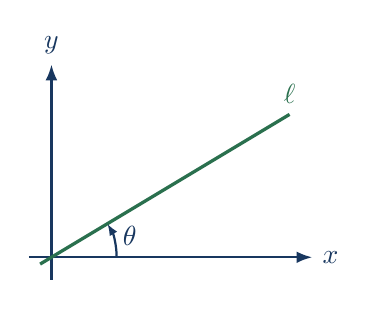
\begin{tikzpicture}[scale=0.72]
			\draw[-{Latex[length=2mm]},AcademicBlue,thick] (-0.4,0)--(4.6,0) node[right] {$x$};
			\draw[-{Latex[length=2mm]},AcademicBlue,thick] (0,-0.4)--(0,3.4) node[above] {$y$};
			\draw[SolutionGreen,very thick] (-0.2,-0.12)--(4.2,2.52) node[above] {$\ell$};
			\draw[AcademicBlue,thick,-{Latex[length=1.5mm]}] (1.15,0) arc[start angle=0,end angle=31,radius=1.15];
			\node[AcademicBlue] at (1.38,0.38) {$\theta$};
		\end{tikzpicture}
	\end{columns}
	\source{Riddle (1982)}
\end{frame}

\begin{frame}[shrink=7]{Gradien menyatakan laju perubahan vertikal terhadap horizontal}
	\begin{block}{Definisi 7 -- Gradien}
		Untuk garis tak vertikal dengan inklinasi $\theta$, \textbf{gradien}
		atau kemiringan garis didefinisikan sebagai
		\[
		\boxed{m=\tan\theta}.
		\]
	\end{block}
	
	\renewcommand{\arraystretch}{1.35}
	\begin{tabular}{>{\centering\arraybackslash}p{0.21\textwidth}
			>{\centering\arraybackslash}p{0.21\textwidth}
			p{0.49\textwidth}}
		\toprule
		Inklinasi & Gradien & Perilaku garis dari kiri ke kanan\\
		\midrule
		$0^\circ<\theta<90^\circ$ & $m>0$ & naik\\
		$\theta=0^\circ$ & $m=0$ & horizontal\\
		$90^\circ<\theta<180^\circ$ & $m<0$ & turun\\
		$\theta=90^\circ$ & tidak terdefinisi & vertikal\\
		\bottomrule
	\end{tabular}
	
	\begin{alertblock}{Catatan}
		Garis vertikal memiliki inklinasi $90^\circ$, tetapi tidak memiliki
		gradien karena $\tan 90^\circ$ tidak terdefinisi.
	\end{alertblock}
\end{frame}

\begin{frame}{Teorema 6 -- Gradien melalui dua titik}
	\begin{block}{Teorema}
		Jika garis tak vertikal melalui dua titik berbeda
		$P_1=(x_1,y_1)$ dan $P_2=(x_2,y_2)$, maka
		\[
		\boxed{m=\frac{y_2-y_1}{x_2-x_1}},\qquad x_1\neq x_2.
		\]
	\end{block}
	
	\begin{columns}[T]
		\column{0.55\textwidth}
		Besaran
		\[
		\Delta x=x_2-x_1,\qquad \Delta y=y_2-y_1
		\]
		masing-masing disebut perubahan horizontal dan perubahan vertikal.
		Dengan demikian,
		\[
		m=\frac{\Delta y}{\Delta x}
		=\frac{\textit{rise}}{\textit{run}}.
		\]
		
		\column{0.39\textwidth}
		\centering
		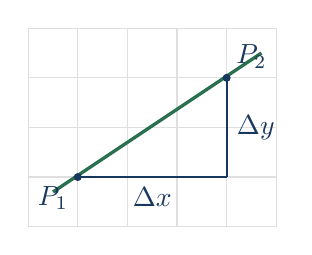
\begin{tikzpicture}[scale=0.63]
			\draw[gray!25,step=1] (0,0) grid (5,4);
			\draw[SolutionGreen,very thick] (0.5,0.7)--(4.7,3.5);
			\fill[AcademicBlue] (1,1) circle (2.3pt) node[below left] {$P_1$};
			\fill[AcademicBlue] (4,3) circle (2.3pt) node[above right] {$P_2$};
			\draw[AcademicBlue,thick] (1,1)--(4,1) node[midway,below] {$\Delta x$};
			\draw[AcademicBlue,thick] (4,1)--(4,3) node[midway,right] {$\Delta y$};
		\end{tikzpicture}
	\end{columns}
\end{frame}

\begin{frame}[shrink=4]{Bukti Teorema 6 dari perbandingan trigonometri}
	Misalkan garis melalui $P_1=(x_1,y_1)$ dan $P_2=(x_2,y_2)$ mempunyai
	inklinasi $\theta$. Translasi titik $P_1$ ke titik asal tidak mengubah
	arah garis. Vektor arahnya menjadi
	\[
	\overrightarrow{P_1P_2}=(x_2-x_1,y_2-y_1)=(\Delta x,\Delta y).
	\]
	
	Karena $\Delta x\neq0$, dari definisi tangen pada segitiga siku-siku
	berarah diperoleh
	\[
	\tan\theta
	=\frac{\text{komponen vertikal}}{\text{komponen horizontal}}
	=\frac{\Delta y}{\Delta x}
	=\frac{y_2-y_1}{x_2-x_1}.
	\]
	Berdasarkan Definisi 7, $m=\tan\theta$. Jadi
	\[
	\boxed{m=\frac{y_2-y_1}{x_2-x_1}}.
	\qquad\square
	\]
	
	\begin{alertblock}{Konsistensi urutan}
		Jika urutan kedua titik dibalik, pembilang dan penyebut sama-sama
		berubah tanda sehingga nilai gradien tetap.
	\end{alertblock}
\end{frame}

\begin{frame}[shrink=5]{Gradien menentukan kesejajaran dan ketegaklurusan}
	\begin{block}{Proposisi 2}
		Untuk dua garis tak vertikal $\ell_1$ dan $\ell_2$ dengan gradien
		$m_1$ dan $m_2$:
		\[
		\begin{aligned}
			\ell_1\parallel\ell_2 &\Longleftrightarrow m_1=m_2,\\
			\ell_1\perp\ell_2 &\Longleftrightarrow m_1m_2=-1.
		\end{aligned}
		\]
	\end{block}
	
	Untuk ketegaklurusan, inklinasi kedua garis berbeda $90^\circ$. Jika
	$\theta_2=\theta_1+90^\circ$, maka
	\[
	m_2=\tan(\theta_1+90^\circ)
	=-\frac{1}{\tan\theta_1}=-\frac1{m_1},
	\]
	sehingga $m_1m_2=-1$.
	
	\begin{alertblock}{Kasus khusus}
		Garis horizontal dan garis vertikal saling tegak lurus, meskipun
		gradien garis vertikal tidak terdefinisi.
	\end{alertblock}
\end{frame}

\begin{frame}{Latihan 7 -- Menentukan gradien dan inklinasi}
	\begin{block}{Soal}
		Garis $\ell$ melalui titik $A=(-2,1)$ dan $B=(4,4)$.
		\begin{enumerate}
			\item Tentukan gradien garis $\ell$.
			\item Tentukan inklinasi $\theta$ dalam derajat.
			\item Jelaskan apakah garis naik atau turun dari kiri ke kanan.
		\end{enumerate}
	\end{block}
	
	\vspace{0.35cm}
	\centering
	\color{AcademicBlue}\bfseries Hitung $\Delta x$ dan $\Delta y$, kemudian gunakan
	$m=\Delta y/\Delta x$ dan $m=\tan\theta$.
\end{frame}

\begin{frame}[shrink=7]{Latihan 7 -- Soal dan pembahasan}
	\begin{exampleblock}{Soal}
		Tentukan gradien dan inklinasi garis melalui $A=(-2,1)$ dan $B=(4,4)$.
	\end{exampleblock}
	
	\[
	\Delta x=4-(-2)=6,\qquad \Delta y=4-1=3.
	\]
	Maka
	\[
	m=\frac{\Delta y}{\Delta x}=\frac36=\boxed{\frac12}.
	\]
	Karena $m>0$, inklinasi berada pada interval $(0^\circ,90^\circ)$, sehingga
	\[
	\theta=\arctan\left(\frac12\right)
	\approx\boxed{26.565^\circ}.
	\]
	
	\begin{exampleblock}{Interpretasi}
		Setiap perpindahan $2$ satuan ke kanan diikuti kenaikan $1$ satuan;
		jadi garis naik dari kiri ke kanan.
	\end{exampleblock}
\end{frame}

\begin{frame}{Latihan 8 -- Gradien negatif dan garis vertikal}
	\begin{block}{Soal}
		Diberikan garis $g$ melalui $P=(-1,3)$ dan $Q=(2,-3)$, serta garis
		$h$ melalui $R=(1,-2)$ dan $S=(1,4)$.
		\begin{enumerate}
			\item Tentukan gradien dan inklinasi garis $g$.
			\item Tentukan inklinasi dan keberadaan gradien garis $h$.
			\item Jelaskan perbedaan geometris kedua garis.
		\end{enumerate}
	\end{block}
	
	\vspace{0.25cm}
	\centering
	\color{AcademicBlue}\bfseries Perhatikan tanda $m$ dan kemungkinan $\Delta x=0$.
\end{frame}

\begin{frame}[shrink=7]{Latihan 8 -- Soal dan pembahasan}
	\begin{exampleblock}{Garis $g$ melalui $P=(-1,3)$ dan $Q=(2,-3)$}
		\[
		m_g=\frac{-3-3}{2-(-1)}=\frac{-6}{3}=-2.
		\]
		Karena $m_g<0$, inklinasi berada pada kuadran II:
		\[
		\theta_g=180^\circ+\arctan(-2)
		\approx\boxed{116.565^\circ}.
		\]
	\end{exampleblock}
	
	\begin{exampleblock}{Garis $h$ melalui $R=(1,-2)$ dan $S=(1,4)$}
		Karena $\Delta x=1-1=0$, garis $h$ vertikal. Jadi
		\[
		\boxed{\theta_h=90^\circ},\qquad
		\boxed{m_h\text{ tidak terdefinisi}}.
		\]
	\end{exampleblock}
\end{frame}

\begin{frame}{Ringkasan teorema utama}
	\renewcommand{\arraystretch}{1.45}
	\begin{tabular}{>{\bfseries}p{0.25\textwidth}p{0.67\textwidth}}
		\toprule
		Konsep & Hasil utama\\
		\midrule
		Jarak rectangular &
		$d=\sqrt{(x_2-x_1)^2+(y_2-y_1)^2}$\\
		Jarak oblique &
		$d^2=(\Delta x)^2+(\Delta y)^2+2\Delta x\Delta y\cos\omega$\\
		Titik tengah &
		$M=\left(\frac{x_1+x_2}{2},\frac{y_1+y_2}{2}\right)$\\
		Pembagi $m:n$ &
		$P=\left(\frac{nx_1+mx_2}{m+n},\frac{ny_1+my_2}{m+n}\right)$\\
		Inklinasi dan gradien &
		$m=\tan\theta=\dfrac{y_2-y_1}{x_2-x_1}$, $0^\circ\leq\theta<180^\circ$\\
		Lingkaran &
		$(x-a)^2+(y-b)^2=r^2$\\
		\bottomrule
	\end{tabular}
	
	\vspace{0.25cm}
	\begin{alertblock}{Struktur Pembuktian}
		Definisi koordinat $\rightarrow$ selisih komponen $\rightarrow$
		rumus analitik $\rightarrow$ interpretasi geometris.
	\end{alertblock}
\end{frame}
% 37
%\begin{frame}{GeoGebra digunakan untuk verifikasi, bukan pembuktian}
%    \begin{enumerate}
%        \item Turunkan dahulu persamaan dari definisi atau teorema.
%        \item Masukkan persamaan pada \textit{GeoGebra Graphing Calculator}.
%        \item Plot titik uji dan periksa apakah titik terletak pada grafik.
%        \item Bandingkan keluaran visual dengan hasil substitusi aljabar.
%    \end{enumerate}
%
%    \begin{block}{Objek yang dapat diverifikasi}
%        \[
%            y=x,
%            \qquad
%            (x-2)^2+(y+1)^2=9,
%            \qquad
%            Q=(5,-1).
%        \]
%    \end{block}
%
%    \begin{alertblock}{Batas Penggunaan}
%        Gambar mendukung intuisi, tetapi kebenaran umum tetap ditentukan oleh pembuktian.
%    \end{alertblock}
%\end{frame}

% 38
%\begin{frame}{Referensi}
%    \begin{thebibliography}{9}
%        \bibitem{Riddle1982}
%        Riddle, D. F. (1982).
%        \newblock \textit{Analytic Geometry} (3rd ed.).
%        \newblock Wadsworth Publishing Company.
%
%        \bibitem{RPS}
%        Departemen Matematika ITS.
%        \newblock \textit{Rencana Pembelajaran Semester SM234102 Geometri Analitik}.
%
%        \bibitem{Fahim2022}
%        Fahim, K. (2022).
%        \newblock \textit{Minggu 1: Titik dan Posisi Titik}.
%        \newblock Departemen Matematika, Institut Teknologi Sepuluh Nopember.
%
%        \bibitem{GeoGebra}
%        GeoGebra.
%        \newblock \textit{Graphing Calculator}.
%    \end{thebibliography}
%\end{frame}

% 39
%\begin{frame}{Ringkasan teorema utama}
%    \renewcommand{\arraystretch}{1.45}
%    \begin{tabular}{>{\bfseries}p{0.25\textwidth}p{0.67\textwidth}}
%        \toprule
%        Konsep & Hasil utama\\
%        \midrule
%        Jarak rectangular &
%        $d=\sqrt{(x_2-x_1)^2+(y_2-y_1)^2}$\\
%        Jarak oblique &
%        $d^2=(\Delta x)^2+(\Delta y)^2+2\Delta x\Delta y\cos\omega$\\
%        Titik tengah &
%        $M=\left(\frac{x_1+x_2}{2},\frac{y_1+y_2}{2}\right)$\\
%        Pembagi $m:n$ &
%        $P=\left(\frac{nx_1+mx_2}{m+n},\frac{ny_1+my_2}{m+n}\right)$\\
%        Lingkaran &
%        $(x-a)^2+(y-b)^2=r^2$\\
%        \bottomrule
%    \end{tabular}
%
%    \vspace{0.25cm}
%    \begin{alertblock}{Struktur Pembuktian}
%        Definisi koordinat $\rightarrow$ selisih komponen $\rightarrow$
%        rumus analitik $\rightarrow$ interpretasi geometris.
%    \end{alertblock}
%\end{frame}

\end{document}
